% Compilar a partir da raiz do projeto, depois de gerar a tabela e a figura:
% Rscript model/verificar_crossing_demanda_ia.R
% latexmk -pdf -outdir=output/pdf model/mudanca_estrutural_ia_democracia.tex
\documentclass[11pt,a4paper]{article}
\usepackage[T1]{fontenc}
\usepackage[utf8]{inputenc}
\usepackage[brazilian]{babel}
\usepackage{lmodern,amsmath,amssymb,booktabs,graphicx,xcolor}
\usepackage[margin=2.45cm,top=2.35cm,bottom=2.35cm]{geometry}
\usepackage{caption,fancyhdr,hyperref}
\definecolor{tinta}{HTML}{172E3B}
\definecolor{azul}{HTML}{22576C}
\hypersetup{colorlinks=true,linkcolor=azul,urlcolor=azul,
  pdftitle={Mudança estrutural induzida por IA e sobrevivência democrática},
  pdfsubject={Esboço de um modelo com demanda não homotética e competição eleitoral}}
\captionsetup{font=small,labelfont=bf,labelsep=period,skip=5pt,hypcap=false}
\setlength{\parindent}{0pt}
\setlength{\parskip}{5.5pt plus 0.7pt minus 0.4pt}
\setlength{\headheight}{15pt}
\setlength{\abovedisplayskip}{7pt}
\setlength{\belowdisplayskip}{7pt}
\pagestyle{fancy}
\fancyhf{}
\fancyhead[L]{\small\sffamily\color{azul}Mudança estrutural e democracia}
\fancyfoot[R]{\small\sffamily\thepage}
\renewcommand{\headrulewidth}{0pt}
\fancypagestyle{primeira}{\fancyhf{}\fancyfoot[R]{\small\sffamily\thepage}}
\newcommand{\titulo}[1]{\section*{\color{tinta}#1}}
\newcommand{\subtitulo}[1]{\par\smallskip{\large\bfseries\color{azul}#1\par}\nobreak}
\newcommand{\Mzero}{M_0}
% Dentro do alinhamento, a entrada primitiva conserva a posição de \bottomrule.
\makeatletter
\newcommand{\linhastabela}{\@@input figures/crossing_demanda_tabela.tex }
\makeatother
\begin{document}
\thispagestyle{primeira}
{\small\sffamily\color{azul}Nota de modelagem\hfill 23 de novembro de 2026\par}
\vspace{5pt}
{\LARGE\bfseries\color{tinta}Mudança estrutural induzida por IA\\[2pt]e sobrevivência democrática\par}
\vspace{5pt}

Uma mesma inovação pode levar um governante a restringir a competição eleitoral ou a preservá-la. No exemplo, a IA reduz a influência de quem permanece no setor automatizado. A demanda desloca trabalhadores para um serviço em que conseguem se organizar com mais eficácia. Conforme a intensidade desse deslocamento, a federação ganha ou perde capacidade de defender as eleições. O emprego total é o mesmo nos dois cenários.

\subtitulo{Um exemplo com o mesmo choque}
Uma unidade do bem automatizável passa a exigir 0,64 unidade de trabalho, frente a uma unidade antes da IA. Uma unidade de serviço continua exigindo uma unidade de trabalho. No ponto de partida, os serviços empregam um quarto da população. Os dois cenários partem dos mesmos preços, quantidades e instituições. No primeiro, a preços fixos, cada real adicional é gasto nas mesmas proporções. No segundo, a demanda por serviços cresce mais do que proporcionalmente à renda. Em ambos, os preços relativos também mudam.

\begin{center}
\captionof{table}{Emprego em serviços, capacidade de organização e decisão do governante.}
\small\renewcommand{\arraystretch}{1.14}\setlength{\tabcolsep}{4.7pt}
\begin{tabular}{@{}lrrrl@{}}\toprule
Cenário & Serviços (\%) & Capacidade \(M\) & Custo de defesa & Equilíbrio\\ \midrule
\linhastabela
\bottomrule\end{tabular}
\end{center}
{\small A federação de trabalhadores aceita pagar até \(V=0{,}90\) para preservar as eleições. O custo da defesa na tabela é o mínimo que ela precisaria pagar se o governante apresentasse a proposta. Valores ilustrativos.}

\begin{center}
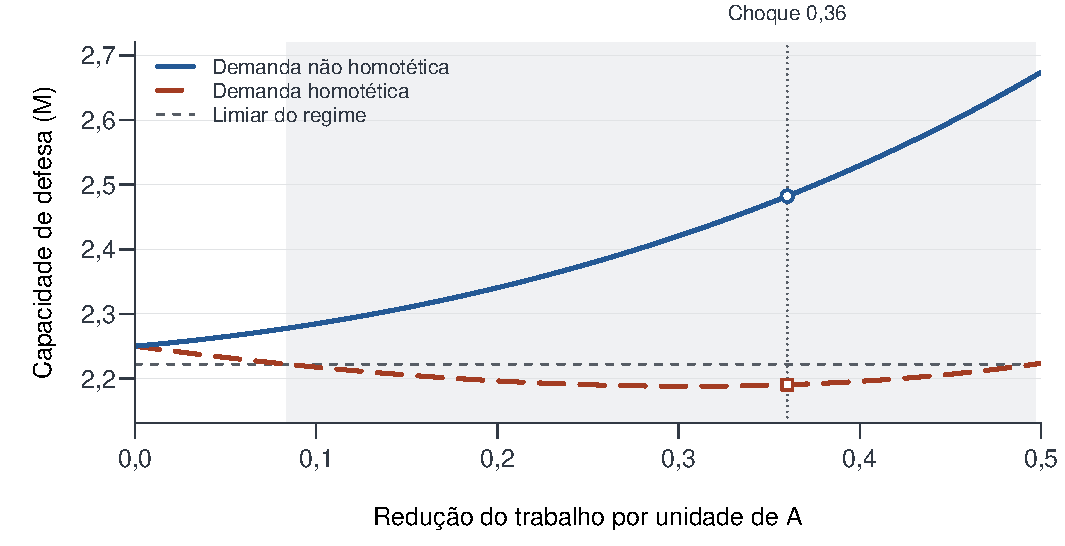
\includegraphics[width=0.94\linewidth]{figures/crossing_demanda_ia.pdf}
\captionof{figure}{Capacidade política conforme cai o trabalho necessário para produzir o bem automatizável. Na faixa cinza, as decisões sobre as eleições divergem. Cada ponto compara uma escolha a partir de uma democracia.}
\end{center}

\newpage
\titulo{1\quad Da cesta de consumo ao emprego}
Há uma unidade de trabalho móvel, um bem automatizável \(A\) e um serviço \(S\). Cada unidade de \(A\) exige tarefas que, inicialmente, consomem o mesmo tempo humano. A IA executa a fração \(a\in[0,1)\) dessas tarefas e está disponível sem custo marginal. As quantidades produzidas são \(y_A=L_A/(1-a)\) e \(y_S=L_S\), com \(L_A+L_S=1\). Com concorrência e salário como numerário, \(w=1\), os preços são \(p_A=1-a\) e \(p_S=1\). A despesa da família representativa é sua renda salarial, \(E=1\).

Como \(p_Ay_A=L_A\) e \(p_Sy_S=L_S\), a parcela de gasto de cada setor coincide com sua parcela de emprego. Escrevemos \(s=L_S\). Assim, a demanda determina quem trabalha onde, preservando o pleno emprego. A mesma cesta física tem o mesmo custo nos dois cenários para qualquer \(a\), pois preços e orçamento coincidem. O índice de utilidade de cada família depende de suas preferências.

\subtitulo{O contrafactual da demanda}
Usamos a função de dispêndio de Comin, Lashkari e Mestieri com dois setores e elasticidade de substituição constante (CES). Seja \(C\) um índice de consumo real, \(s_0\in(0,1)\) a parcela inicial dos serviços e \(r=1-\sigma\in(0,1)\), onde \(\sigma\) é a elasticidade de substituição. Normalizamos o parâmetro de não homoteticidade de \(A\) em 1 e denotamos o de \(S\) por \(\eta\). O dispêndio mínimo \(\mathcal E_\eta\) satisfaz
\begin{equation}
  \mathcal E_\eta(C,p)^r=(1-s_0)p_A^r C^r+s_0p_S^r C^{r\eta}.
\end{equation}
Com \(\eta=1\), a demanda é homotética. Com \(\eta>1\), os serviços ganham participação quando cresce a renda a preços fixos. A elasticidade-renda observável de \(S\) no ponto de partida vale \(\xi_S=\sigma+r\eta/(1-s_0+s_0\eta)\). No exemplo, \(\eta=6\) corresponde a \(\xi_S=1{,}67\). A forma funcional e a expressão para a elasticidade vêm das equações 3 e 9 do artigo. \href{https://dcomin.host.dartmouth.edu/Publications_files/ECTA16317.pdf}{Comin, Lashkari e Mestieri (2021), pp.~317--319.}

Em equilíbrio, \(\mathcal E_\eta=1\) e a demanda hicksiana implica \(s=s_0 C^{r\eta}\). Eliminando \(C\), basta resolver
\begin{equation}
  1-s=(1-s_0)(1-a)^r\left(\frac{s}{s_0}\right)^{1/\eta}. \label{eq:share}
\end{equation}
O lado esquerdo cai com \(s\) e o direito sobe. Quando \(a>0\), a solução única está entre \(s_0\) e 1. Para esse intervalo, aumentar \(\eta\) reduz o lado direito a \(s\) fixo e eleva o emprego de equilíbrio nos serviços. Em particular,
\[
 s_H(a)=\frac{s_0}{s_0+(1-s_0)(1-a)^r}<s_N(a) \quad(a>0),
\]
com \(H\) para \(\eta=1\) e \(N\) para \(\eta>1\). A queda do preço de \(A\) já desloca parte do gasto para \(S\) em \(H\) porque \(\sigma<1\).

Podemos isolar o efeito-renda diretamente. Aos novos preços, dê à família exatamente o orçamento \(E_c=\mathcal E_\eta(1,p)<1\) que permite manter o consumo real inicial. Por (1), \(E_c^r=(1-s_0)(1-a)^r+s_0\) nas duas especificações. A parcela compensada de gasto em serviços também é idêntica, \(s_0/E_c^r=s_H(a)\). Ao restaurar o orçamento efetivo \(E=1\), a parcela fica em \(s_H\) na demanda homotética e sobe a \(s_N\) na não homotética. Todo o diferencial \(s_N-s_H\) nesse experimento vem do uso do ganho de poder de compra.

\newpage
\titulo{2\quad Quando uma restrição eleitoral compensa}
O regime inicial tem eleições competitivas. Os jogadores são o governante e uma federação que representa os trabalhadores dos dois setores. A federação atribui valor \(V>0\) à possibilidade de alternância, por exemplo, porque futuros governos podem reverter decisões desfavoráveis aos trabalhadores. O governante ganha \(G>0\) se restringir a competição. \(V\) e \(G\) são comuns aos dois cenários. Todos observam o choque, as participações no emprego e os parâmetros políticos.

\begin{enumerate}\setlength{\itemsep}{2pt}
\item O governante mantém as regras, com payoffs \((0,V)\), ou apresenta uma proposta de restrição ao custo \(f\), com \(0<f<G\).
\item Se há proposta, a federação escolhe quanto esforço \(e_j\geq0\) dedicar por trabalhador de cada setor \(j\in\{A,S\}\). Esse esforço tem custo \(K=\tfrac12\sum_j L_j c_j e_j^2\), com \(c_j>0\). Ele gera oposição de intensidade \(Z=\sum_j L_j d_j e_j\), com \(d_j>0\).
\item O governante observa \(Z\) e implementa a restrição, recebendo \(G-Z-f\), ou retira a proposta, recebendo \(-f\). Na igualdade \(Z=G\), prevalece a regra eleitoral vigente. O payoff da federação é \(V-K\) se as eleições continuam competitivas e \(-K\) se a restrição é implementada.
\end{enumerate}

O parâmetro \(c_j\) mede o custo de coordenar trabalhadores no setor. O parâmetro \(d_j\) mede quanto a ação coordenada desses trabalhadores pesa no cálculo do governo, por exemplo, pela dependência de seus apoiadores em relação à cooperação do setor. A federação já dispõe de representação nos dois setores. Seus esforços são escolhas posteriores à produção e têm custo em utilidade política.

\subtitulo{Solução por indução retroativa}
No último estágio, basta alcançar \(Z=G\) para obter a retirada. Se esse objetivo for caro demais, o melhor esforço é zero. Para encontrar a alternativa de menor custo, defina
\[
 b_j=\frac{d_j^2}{c_j},\qquad M=(1-s)b_A+s b_S.
\]
A desigualdade de Cauchy--Schwarz dá \(Z^2\leq 2KM\). Ela vale como igualdade para \(e_j^*=Gd_j/(c_jM)\). Logo, a defesa custa \(K^*=G^2/(2M)\). A federação a empreende se \(V>K^*\). O governante antecipa essa escolha e preserva as regras para poupar \(f\). Se \(V<K^*\), ele apresenta e implementa a restrição, recebendo \(G-f>0\). Assim, no equilíbrio perfeito em subjogos, fora da igualdade,
\begin{equation}
  M>\tau \ \Longrightarrow\ \text{eleições preservadas},\qquad
  M<\tau \ \Longrightarrow\ \text{competição restrita},
  \qquad \tau=\frac{G^2}{2V}. \label{eq:tau}
\end{equation}
O desempate em \(Z=G\) garante que o esforço mínimo basta para obter a retirada. Em \(M=\tau\), a federação é indiferente e ambas as decisões de regime são compatíveis com equilíbrio. Nos dois ramos estritos, o esforço observado em equilíbrio é zero. Sua credibilidade determina a escolha do governante antes de qualquer mobilização.

\newpage
\titulo{3\quad Duas condições de inversão}
Suponha \(d_A(a)=d_{A0}(1-\rho a)\), com \(0\leq\rho<1\). Quanto mais a IA substitui a cooperação humana no setor \(A\), menor a influência de um esforço realizado ali. Esse é um \emph{pressuposto político} que pode ser testado separadamente do ganho de produtividade. Escreva \(b_0=d_{A0}^2/c_A\). Assim \(b_A(a)=b_0(1-\rho a)^2\). A capacidade por trabalhador \(b_S\) do setor de serviços permanece constante.

\subtitulo{A escolha institucional depois do choque}
Como os dois cenários têm os mesmos \(b_j\) para todo \(a\), a diferença de capacidade é exatamente
\begin{equation}
 M_N(a)-M_H(a)=[s_N(a)-s_H(a)]\,[b_S-b_A(a)]. \label{eq:gap}
\end{equation}
O gasto adicional em serviços fortalece a defesa das eleições se os trabalhadores que entram no setor ganham capacidade política por pessoa. Se \(b_S<b_A(a)\), ele a enfraquece. Se as capacidades setoriais coincidem, o efeito de composição é zero mesmo que o emprego mude muito.

Seja \(\Mzero=(1-s_0)b_0+s_0b_S\). O resultado anunciado requer, para algum \(a>0\),
\begin{equation}
 M_H(a)<\tau<\min\{\Mzero,M_N(a)\}. \label{eq:cross}
\end{equation}
A primeira desigualdade dá a restrição sob demanda homotética. As demais dão eleições preservadas no ponto de partida e no cenário não homotético. As desigualdades estritas sobrevivem a pequenas perturbações dos parâmetros. Com \(b_S>b_A(a)\), a participação crítica é \(s_c=(\tau-b_A(a))/(b_S-b_A(a))\), quando esse valor está entre zero e um.

\subtitulo{O sinal do efeito da automação}
Uma diferença na escolha de regime pode ocorrer mesmo que os dois cenários percam capacidade. Uma segunda questão é se o choque reduz \(M_H\) e aumenta \(M_N\). A resposta local independe da distância ao limiar institucional. Na origem, a diferenciação de \eqref{eq:share} dá
\begin{align}
 s'_\eta(0)&=r\,s_0(1-s_0)\frac{\eta}{1-s_0+s_0\eta},\\
 M'_\eta(0)&=(b_S-b_0)s'_\eta(0)-2\rho(1-s_0)b_0.
\end{align}
O primeiro termo é o ganho ou perda pela mudança de setor. O segundo é a perda de influência de quem permanece em \(A\). Quando \(b_S>b_0\), há inversão local de sinal precisamente se
\[
 (b_S-b_0)s'_1(0)<2\rho(1-s_0)b_0<(b_S-b_0)s'_\eta(0).
\]
No exemplo, \(M'_H(0)=-0{,}375\) e \(M'_N(0)=+0{,}250\). Mantendo os outros parâmetros, a mudança de sinal exige \(\eta>3\), ou \(\xi_S>1{,}40\) na origem. Para \(\eta_N=6\), a inversão local ocorre quando \(4{,}75<b_S<11\), com \(b_0=1\). A intensidade organizacional do setor de destino é, portanto, uma hipótese quantitativamente relevante.

Também é possível delimitar a faixa cinza da Figura 1. Em qualquer \(a\), a derivada satisfaz
\[
 \frac{M'_\eta(a)}{1-s}=
 r\frac{\eta s}{1-s+\eta s}\frac{b_S-b_A(a)}{1-a}-2\rho b_0(1-\rho a).
\]
No exemplo, o lado direito cresce estritamente com \(a\), pois \(s\) sobe, \(b_S>b_0\) e \(b_A\) cai. Ele tende a \(+\infty\) quando \(a\) se aproxima de 1. Assim, \(M_N\) cresce desde a origem, e \(M_H\) tem um único mínimo. São os dois encontros de \(M_H\) com o limiar institucional que delimitam a faixa de decisões divergentes.

\newpage
\titulo{4\quad Interpretação e sensibilidade}
\subtitulo{Quanto emprego precisa mudar de setor?}
No exemplo, \(s_0=0{,}25\), \(\sigma=0{,}60\), \(\rho=0{,}50\), \(b_0=1\), \(b_S=6\), \(G=2\), \(V=0{,}90\) e \(f=0{,}10\). Tomamos \(c_A=c_S=1\). No choque \(a=0{,}36\), a parcela crítica é \(s_c\simeq29{,}1\%\). Substituí-la em \eqref{eq:share} determina a intensidade de não homoteticidade necessária para atingir esse ponto,
\[
 \eta_{\rm regime}=
 \frac{\log(s_c/s_0)}{\log\!\left[(1-s_c)/((1-s_0)(1-a)^r)\right]} .
\]
A expressão dá um limiar interior quando \(s_H(a)<s_c<1-(1-s_0)(1-a)^r\). Na ilustração, \(\eta_{\rm regime}=1{,}238\), ou \(\xi_S\simeq1{,}067\) na origem. Para \(1{,}238<\eta<1{,}471\), a democracia sobrevive ao choque mesmo tendo perdido capacidade política em relação ao ponto de partida (limites arredondados). Com \(\eta_N=6\), a escolha de regime diverge nos choques entre \(a\simeq0{,}0834\) e \(0{,}4967\). Quando \(a\) tende a 1, ambos os cenários concentram o emprego em \(S\) e \(M\) tende a \(b_S\). Esses contrafactuais descrevem a decisão em uma democracia existente.

\subtitulo{Três mudanças nas regras do jogo}
\textbf{Mobilização anterior à proposta.} Se a federação tem de pagar pela mobilização antes de o governante decidir, ele só propõe quando \(G-Z-f>0\). Com status quo no empate, basta \(Z=G-f\) e o limiar cai para \((G-f)^2/(2V)\). Com \(f=0{,}10\), ambos os cenários preservam as eleições no choque da Tabela 1. Com \(f=0{,}005\), volta a haver inversão. A ordem das decisões pode mudar a previsão institucional mesmo quando a realocação do emprego é idêntica.

\textbf{Valor privado das eleições.} Suponha que só a federação conheça \(V\), com distribuição contínua e conhecida. Dado \(M\), o governante propõe se \(G\Pr(V<K^*)>f\), pois a proposta rende \(-f\) diante de uma defesa crível. Para qualquer distribuição contínua com suporte em \([0{,}895,0{,}905]\), as decisões da Tabela 1 permanecem estritas para todos os tipos.

\textbf{Custo de organização.} Substitua o custo quadrático por \(K=\sum_j L_j c_j e_j^p/p\), com \(p>1\). A minimização dá \(K^*=G^p/(pM_p^{p-1})\), com \(M_p=\sum_j L_j(d_j^p/c_j)^{1/(p-1)}\). A continuidade em \(p=2\) preserva as escolhas estritas para expoentes suficientemente próximos de 2.

\subtitulo{O que a evidência teria de sustentar}
O parâmetro decisivo é a capacidade de organização dos serviços que \emph{recebem} a demanda adicional. Uma verificação empírica confrontaria elasticidades de gasto e absorção de emprego com medidas independentes de representação coletiva e de influência sobre o governo. O resultado histórico dos três quartos em Comin e coautores não calibra esses parâmetros. O jogo trata da continuidade da competição eleitoral, toma a representação dos trabalhadores como dada e abstrai das rendas dos proprietários da IA. A relação entre o local de trabalho e a organização política, e o efeito da automação sobre a cooperação no trabalho, motivam os dois termos da derivada. \href{https://doi.org/10.1353/wp.2024.a933069}{Van Noort (2024)} e \href{https://economics.mit.edu/sites/default/files/2023-07/Harms\%20of\%20AI.pdf}{Acemoglu, seção 4.4 de \emph{Harms of AI}}. Fontes consultadas em 23/11/2026.
\end{document}
